\chapter{Model of the system}
In order to calculate the participation ratio of the different lossy layers in an arbitrary structure it is simulated using 3D EM simulation software called CST.


\section{Josephson junction}
During simulation in CST, the Josephson junction is replaced by an inductor. By tuning the inductance together with the capacitance of the structure a specific resonance frequency can be reached.


\section{Lossy layers}
The relatively small thickness of the layers suggests that the impact they have on the Electric field is small. During simulation their impact is neglected and the layers are therefore omitted. The exclusion of thin lossy layers prevents the necessity for mesh elements with sub-nano meter size. This significantly reduces the number of mesh elements and in turn the computation time of the simulation. A simple representation of the structure can be seen in figure~\ref{fig:model}.
\begin{figure}
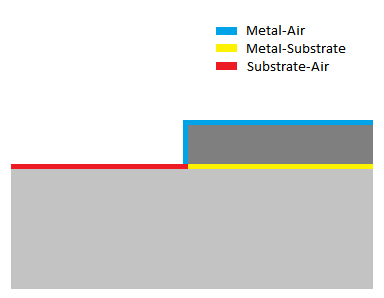
\includegraphics[scale=.8]{Figures/model}
\caption{Simplification of the system including three lossy layers. The substrate and metal are depicted in light and dark grey respectively}
\label{fig:model}
\end{figure}


\section{Ground}
To further reduce the number of mesh elements, the ground pad is replaced by a thin sheet of PEC. Considering the field in the ground region is small compared to the field at the edges of the pads its contribution to the participation ratio is also small. Investing more computation time on the ground region by increasing the density of mesh elements there would therefore also have limited impact on the participation ratio.
\section{title}